\graphicspath{{figs/3b}}

\chapter{Approximate Inference in Classification}
\section{Bayesian Logistic Regression}
\subsection{Maximum-A-Posteriori Estimate}
\paragraph{1.1. Analyze the results provided by \Cref{fig:logreg_map}. Looking at $p(y=1 | x, \mathbf{w}_{\textrm{MAP}})$, what can you say about points far from train distribution?}

Approximating $p(\mathbf{w} | \mathbf{X}, \mathbf{Y})$ with a Dirac delta function is essentially akin to approximating the predictive distribution using $\mathbf{w}_{\textrm{MAP}}$, meaning $p(y=1 | x, \mathbf{w}_{\textrm{MAP}}) \approx p(y=1 | x, \mathbf{Y})$. This approximation is quite rudimentary. As depicted in \Cref{fig:logreg_map}, the model's uncertainty doesn't significantly increase far from the training data. This limitation indicates that the point-wise estimate of the parameters can only confidently assign points to their respective classes but lacks the capacity to provide nuanced uncertainty measures for points that deviate far from the training data distribution. Thus, it lacks in providing uncertainty measures for outlying points.

% The model exhibits a limitation in uncertainty estimation, remaining overconfident far from the training data, hence lacking in providing nuanced uncertainty measures for outlying points.

\begin{figure}[H]
    \centering
    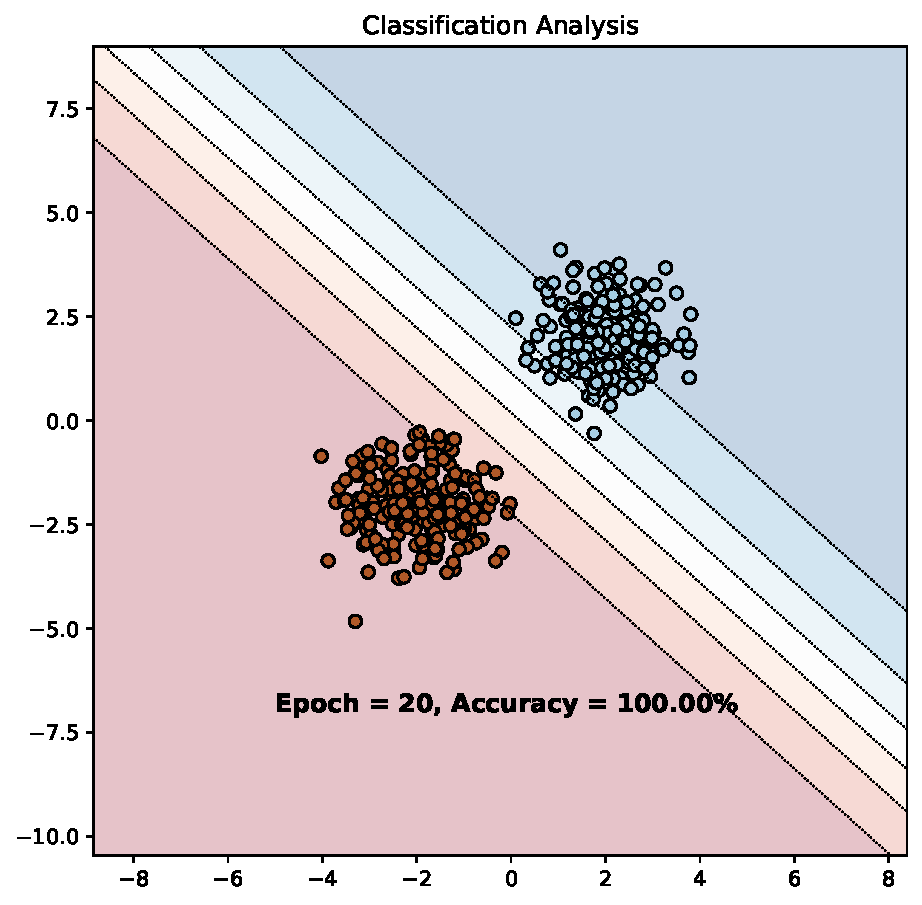
\includegraphics[width=0.45\textwidth]{logreg_map.pdf}
    \caption{Illustration of a Bayesian Logistic Regression model applied to a binary classification task with uncertainty display, with a weight decay of $5 \times 10^{-2}$. Two distinct data point clusters — blue and red — represent separate classes, while the surrounding shaded areas reflect the model's predictive uncertainty, with lighter shades indicating lower confidence.}
    \label{fig:logreg_map}
\end{figure}

\subsection{Laplace Approximation}
\paragraph{1.2. Analyze the results provided by \Cref{fig:laplace_approx}. Compared to previous MAP estimate, how does the predictive distribution behave?}

Compared to the MAP estimate, the predictive distribution in Bayesian Logistic Regression with Laplace approximation captures the uncertainty about the model parameters. While the MAP estimate provides a single point estimate of the weights ($ \mathbf{w}_{\textrm{MAP}} $), thus a single decision boundary, the Laplace approximation models the weights as a normal distribution centered around $ \mathbf{w}_{\textrm{MAP}} $ with a covariance matrix derived from the Hessian of the log posterior, which allows uncertainty in the decision boundary, as clearly displayed in \Cref{fig:laplace_approx}.

\begin{figure}[H]
    \centering
    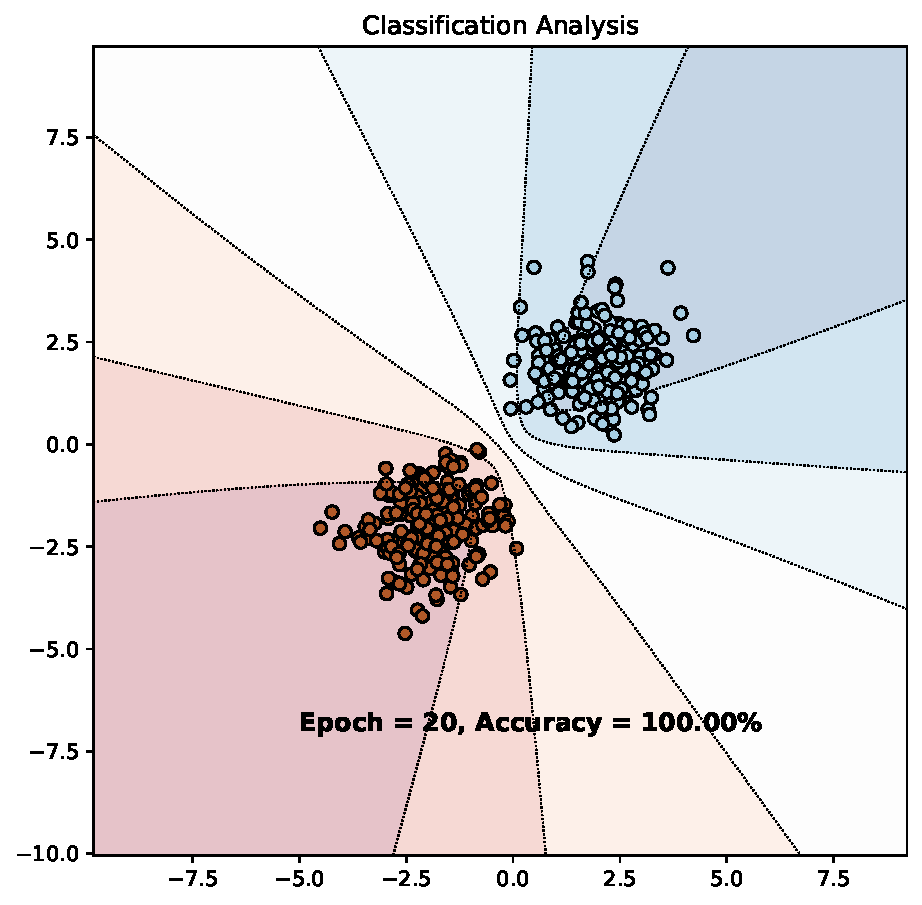
\includegraphics[width=0.45\textwidth]{laplace_approx.pdf}
    \caption{Illustration of a Bayesian Logistic Regression with Laplace approximation model applied to a binary classification task, with a weight decay of $5 \times 10^{-2}$.}
    \label{fig:laplace_approx}
\end{figure}


\paragraph{1.3. Comment the effect of the regularisation hyper-parameter  \texttt{WEIGHT\_DECAY}.}

The weight decay hyper-parameter controls the complexity of the model. It adds a penalty to the loss function for large weights, effectively encouraging the model to maintain smaller weight values. This usually help prevent overfitting by discouraging the model from relying too heavily on any single feature or combination of features.

In Bayesian terms, weight decay corresponds to the precision (inverse variance) of the prior distribution over the weights. A higher weight decay value means a tighter prior, which pulls the weights closer to zero, unless the data provides strong evidence to the contrary. This can affect the predictive distribution by potentially making it more conservative. As a result, the decision boundary may be less flexible and the model may exhibit higher uncertainty, especially in regions far from the training data. This behavior is verified in \Cref{fig:weight_decay}. When the weight decay is too high, it results in increased predictive uncertainty (wider shaded areas), whereas when it's too low, it results in high confidence (narrower shaded areas), which may not be justified for unseen data.

\begin{figure}[H]
    \centering
    \begin{subfigure}{0.45\textwidth}
        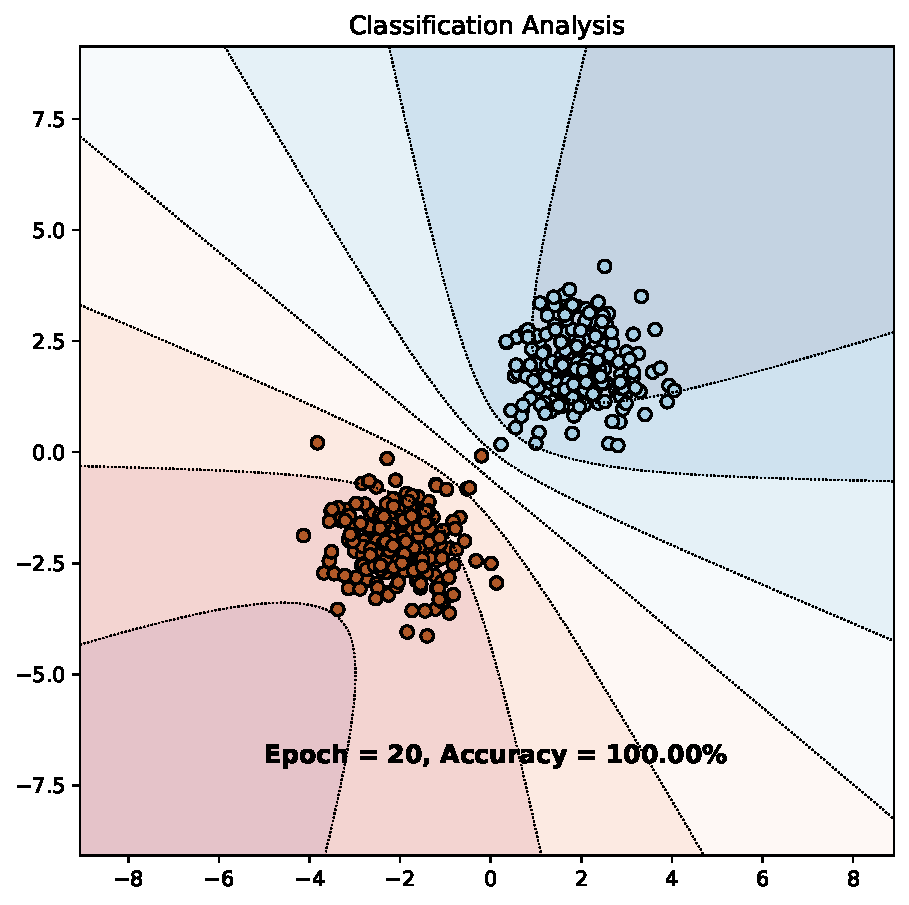
\includegraphics[width=\textwidth]{laplace_approx_0.5.pdf}
        \caption{}
        \label{subfig:weight_decay_high}
    \end{subfigure}%
    \begin{subfigure}{0.45\textwidth}
        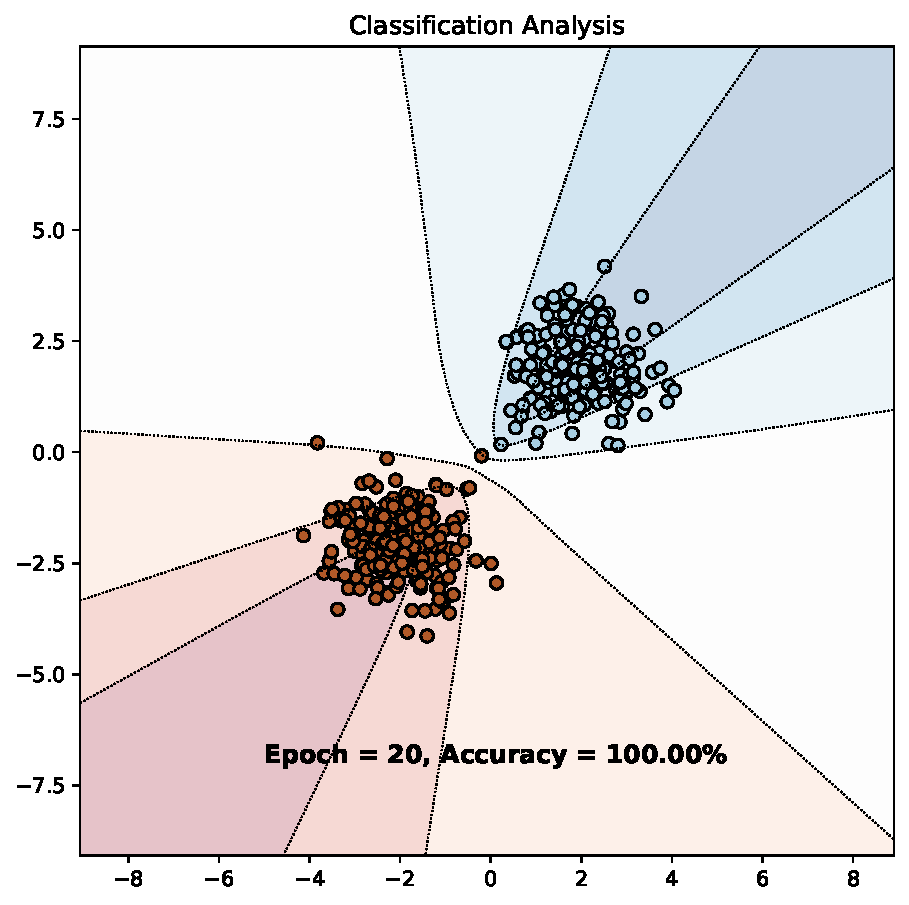
\includegraphics[width=\textwidth]{laplace_approx_5e-05.pdf}
        \caption{}
        \label{subfig:weight_decay_low}
    \end{subfigure}%
    \caption{Illustration of a Bayesian Logistic Regression with Laplace approximation model applied to a binary classification task, with a weight decay of (a) $0.5$ and (b) $5 \times 10^{-5}$.}
    \label{fig:weight_decay}
\end{figure}

\subsection{Variational Inference}
\paragraph{1.4. Comment the code of the \texttt{VariationalLogisticRegression} and \texttt{LinearVariational} classes.}

\noindent\texttt{LinearVariational} represents a single linear layer with variational inference applied. It approximates the weights and biases of the layer with distributions rather than fixed values.
\begin{itemize}
    \item The class is initialized with the variational parameters for the weights (\texttt{w\_mu}, \texttt{w\_rho}) and bias (\texttt{b\_mu}) of the layer, i.e. the parameters we want to learn. \texttt{prio\_var} represents the variance of the prior distribution ($\sigma^2_p$), to specify our prior belief about the distribution of the weights. 
    \item The \texttt{sampling} method uses the reparametrization trick to sample from the variational posterior distribution for the weights. The reparametrization trick allows the gradient of the loss function to backpropagate through the randomness of the sampling process. 
    \item The \texttt{kl\_divergence} method calculates the Kullback-Leibler divergence between the variational posterior and the prior distribution for the weights.
    \item The \texttt{forward} method defines the forward pass by sampling the weights then by computing the output of the layer using the sampled weights and the mean of the biases.
\end{itemize}

\noindent\texttt{VariationalLogisticRegression} represents a logistic regression model using variational inference:
\begin{itemize}
    \item The class is initialized with one linear variational layer used to perform the linear transformation in logistic regression.
    \item The \texttt{forward} method defines the forward pass for the logistic regression model by returning the probabilities of the positive class. 
    \item The \texttt{kl\_divergence} method simply calls the same method of the \texttt{LinearVariational} layer to obtain the KL divergence term for the model.
\end{itemize}

\paragraph{1.5. Comment the code of the training loop, especially the loss computation. Analyze the results provided by \Cref{fig:logreg_variational}. Compared to previous MAP estimate, how does the predictive distribution behave? What is the main difference between the Variational approximation and the Laplace approximation?}

The loss function calculates the Evidence Lower Bound (ELBO), which we want to maximize. In theory, we aim to maximize the likelihood of the data directly, but this is often intractable due to the integral over the weights. Therefore, we compute the Kullback-Leibler divergence between the variational distribution $q_{\theta}(w)$ and the prior distribution $p(w)$. This acts as a regularization term, encouraging the variational distribution to be similar to the prior distribution. It represents the information lost when using $q_{\theta}(w)$ to approximate $p(w)$, which we want to minimize. 

To ensure the model fits the data effectively, we compute the negative log-likelihood of the data under the model parameterized by the weights sampled from $q_{\theta}(w)$. This is done using a binary cross-entropy loss. Subsequently, we employ gradient descent (thus minimizing the negative ELBO) to update the parameters of the variational distribution to better approximate the true posterior.

Compared to a MAP estimate, the variational approach does not just find the most probable weights (as MAP does) but instead approximates the entire posterior distribution over the weights. In the variational approach, the predictive distribution captures the model's uncertainty about its predictions.

\begin{figure}[H]
    \centering
    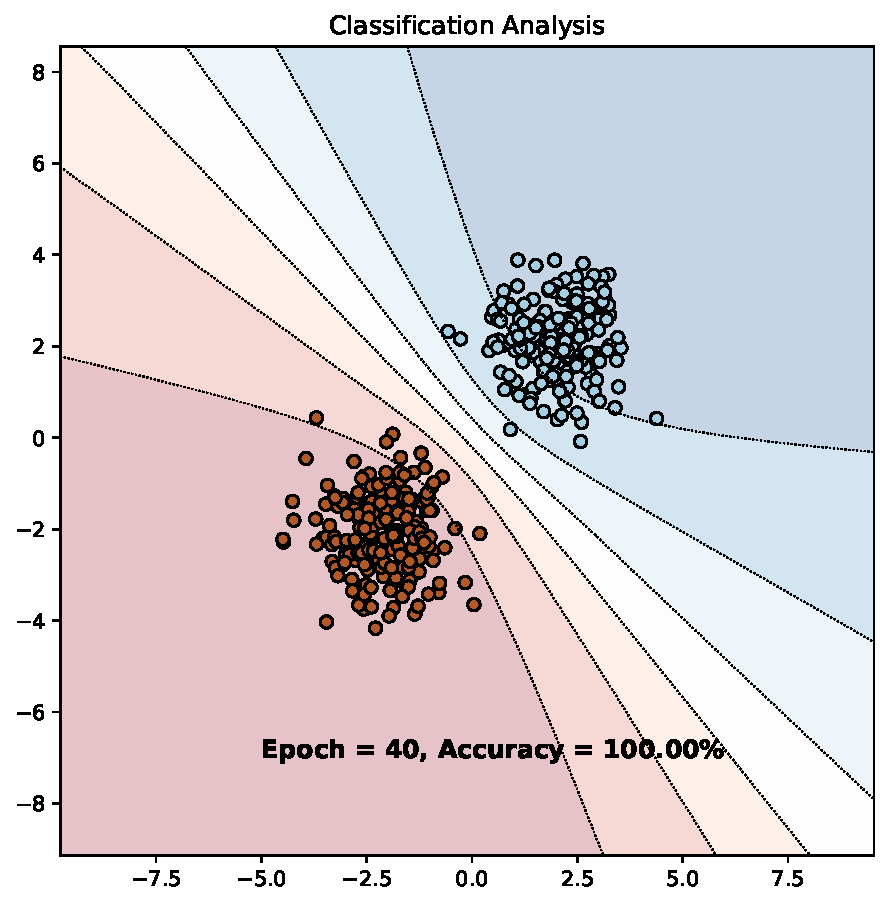
\includegraphics[width=0.45\textwidth]{logreg_variational.pdf}
    \caption{Illustration of a Variational Logistic Regression model applied to a binary classification task.}
    \label{fig:logreg_variational}
\end{figure}

\section{Bayesian Neural Networks}
\subsection{Variational Inference with Bayesian Neural Networks}
\paragraph{2.1. Analyze the results showed on \Cref{fig:mlp_variational}.}

...

\begin{figure}[H]
    \centering
    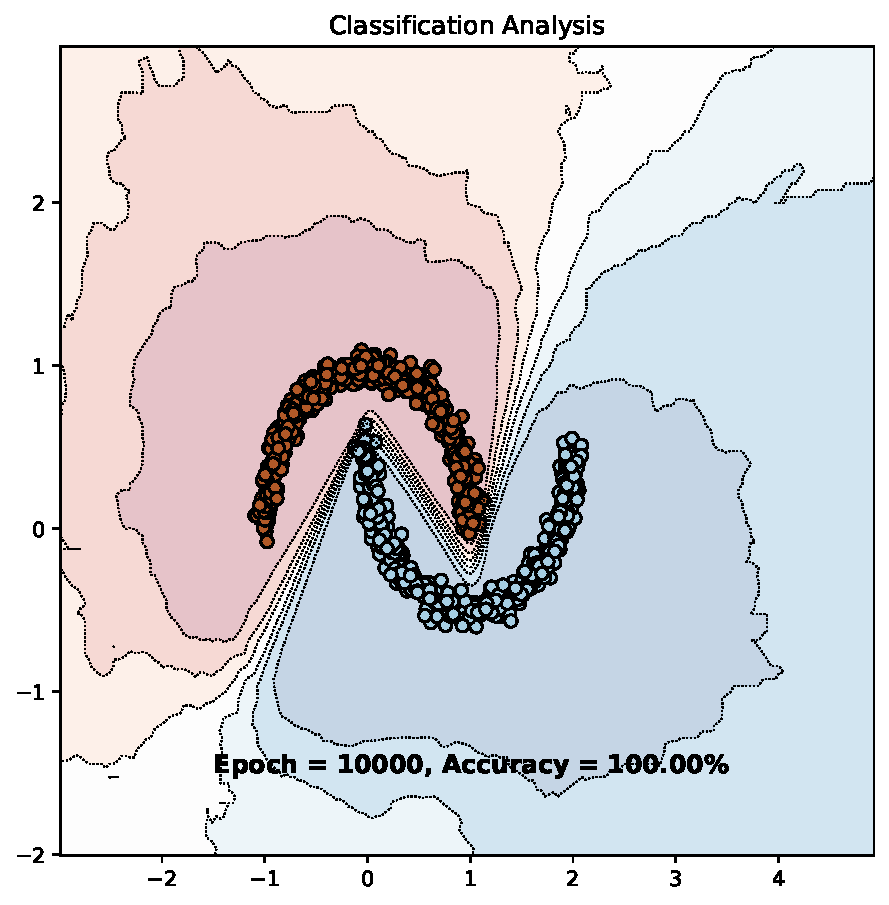
\includegraphics[width=0.45\textwidth]{mlp_variational.pdf}
    \caption{Illustration of a Bayesian Neural Network model applied to a binary classification task.}
    \label{fig:mlp_variational}
\end{figure}


\subsection{Monte Carlo Dropout}
\paragraph{2.2. Again, analyze the results showed on \Cref{fig:dropout}. What is the benefit of MC Dropout variational inference over Bayesian Logistic Regression with variational inference?}

...

\begin{figure}[H]
    \centering
    \begin{subfigure}{0.45\textwidth}
        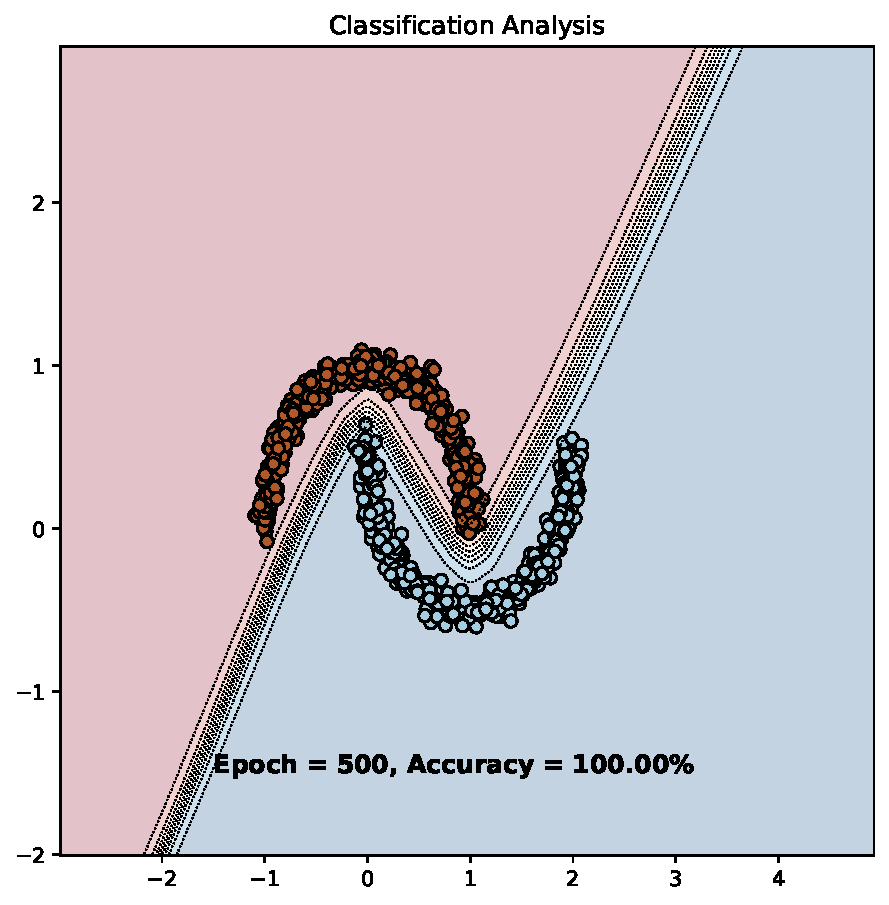
\includegraphics[width=\textwidth]{dropout.pdf}
        \caption{}
    \end{subfigure}%
    \begin{subfigure}{0.45\textwidth}
        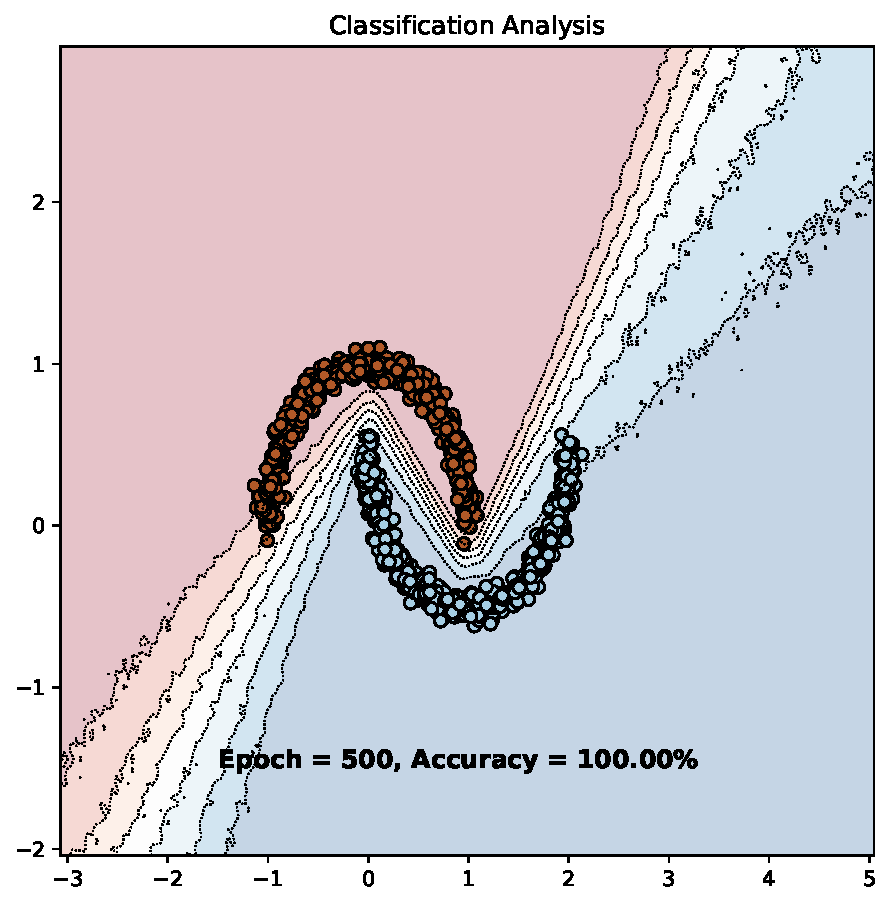
\includegraphics[width=\textwidth]{mcdropout.pdf}
        \caption{}
    \end{subfigure}%
    \caption{Illustration of a Bayesian Neural Network model applied to a binary classification task using (a) dropout and (b) Monte-Carlo dropout.}
    \label{fig:dropout}
\end{figure}
